%%%%%%%%%%%%%%%%%%%%%%%%%%%%%%%%%%%%%%%%%%%%%%%%%%%%%%%%%%%%%%
%%%%% Definiera diverse saker här som används i dokumentet
\newcommand{\TitleText}{Radiohandbok Kortvåg}
\newcommand{\SubtitleText}{För Sändaramatörer\\ och kortvågslyssnare}
\newcommand{\Forfattare}{Täpp-Anders Sikvall}
\newcommand{\Initialer}{SMØUEI}
\newcommand{\DokYear}{19}
\newcommand{\DokVersion}{2.0.0}
\newcommand{\DokumentRevision}{x.y.z}
\newcommand{\DokumentDatum}{\today}
%%%%%%%%%%%%%%%%%%%%%%%%%%%%%%%%%%%%%%%%%%%%%%%%%%%%%%%%%%%%%%%%%%


% Tables are getting a little squashed without this
\renewcommand{\arraystretch}{1.15}

%\titlefootfalse % Använd denna för ren förstasida
\titlefoottrue % Använd denna för en footer på första sidan
%\newcommand{\titlefootcontent}{%
%	\begin{tabularx}{.9\textwidth}{X X X X}	%
%		\textbf{Intressegrupp} & \textbf{Författare} & \textbf{Datum}  & \textbf{Utgåva} \\		%
%		\Mottagare       & \Forfattare          & \DokumentDatum & \DokumentNummer   \\		%            
%	\end{tabularx}%
%}

%\addtolength{\headsep}{3mm}
%\addtolength{\textheight}{15mm}	

%%%%%%%%%%%%%%%%%%%%%%%%%%%%%%%%%%%
%%% Bygger förstasidan här

\newgeometry{left=2cm,right=2cm,bottom=1cm,top=1cm}
\pagestyle{empty}
\vfill
%	\begin{flushright}
%		
\includegraphics[width=0.1\textwidth]{logo/logo}
%	\end{flushright}
\vspace*{4cm}
\centerline{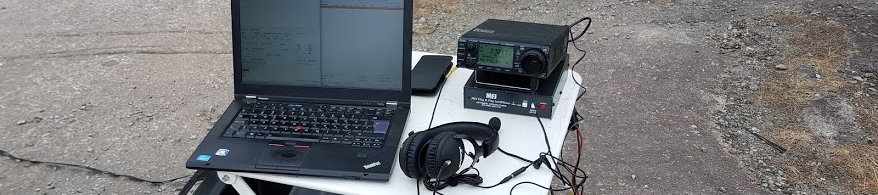
\includegraphics[width=\paperwidth]{logo/rubrikbild}}
\begin{flushright}
	\Huge{\bfseries{\TitleText}} \\[3mm]
	\Large{\bfseries{\SubtitleText}}
\end{flushright}

\vfill

%	\small
%	\begin{tabular}{llll}
%		\textbf{Rev} & \textbf{Date} & \textbf{Responsible} & \textbf{Description}       \\ \hline
%		B            & 2019-03-16    & ANSI                 & Uppdateringar med mer info \\
%		A            & 2019-03-15    & ANSI                 & Initial version
%	\end{tabular}
%	\normalsize 
%	\vfill

%	\iftitlefoot
%	\scriptsize
%	\vspace*{-1em}
%	\hrule
%	\begin{center}
%		\begin{tabularx}{.9\textwidth}{X X X X}
%			\titlefootcontent &
%		\end{tabularx}
%	\end{center}
%	\normalsize
%	\fi
\newpage

%\restoregeometry

\newgeometry{top=3cm}

\pagestyle{fancy}
%\setlength{\headheight}{53pt} 

%	\lhead{
\includegraphics[height=10pt]{logo/logo}}
\lhead{\leftmark}	
\rhead{
	\scriptsize
	\begin{tabular}{ll}
		\textbf{Version} & \textbf{Datum}\\
		\DokVersion & \DokumentDatum\\
	\end{tabular}
}

\chead{}

\lfoot{
	\scriptsize
	www.sm0uei.se
}

\cfoot{\scriptsize \thepage\ / \pageref{LastPage}}

\rfoot{\scriptsize
	anders@sikvall.se
}

\renewcommand{\footrulewidth}{0.2pt}

\widowpenalty=9999
\clubpenalty=9999

%	\setlength{\headsep}{1em}2



%%%%%%%%%%%%%%%%%%%%%%%%%%%%%%%%%%%%%%%%%%%%%%%%%%%%%
%%% Här börjar dokumentet som skall redigeras
%

\cleardoublepage
%\newgeometry{left=3.2cm,right=3.2cm,bottom=2.5cm,top=2.5cm}

%%% Innehållsförteckning
\tableofcontents

\newpage

% Lista bilagor här

%\listoffigures

%\listoftables

%\listoftodos


%%% Justera här om du föredrar indrag som i löpande text. Teknisk dokumentation
%%% tycker jag fungerar bättre med styckenmellanrum utan indrag. \parskip
%%% justerar styckemellanrum och \parindent är indrag.



\setlength{\parskip}{0.5em}
\setlength{\parindent}{0pt}

\section*{Förord}

Det du nu håller i din hand eller läser på din skärm är resultatet av en omarbetning av den tidigare radiohandboken. Denna version kommer sig av att det var dags att uppdatera layouten och även passa på att städa upp lite i boken så att den blev lite mer strukturerad.

Denna del innehåller bara HF. Det finns också en variant som är för VHF/UHF och en version som innehåller hela boken i samma fil.

De tidigare versionerna särskilt tänkta att läsas på platta, ebokläsare eller mobil har utgått. Detta för att de inte var särskilt populära eller ofta nedladdade liksom att det tar en del tid i anspråk att underhålla flera olikva versioner av samma material. Eftersom sidstorleken för läs- och surfplattor är bäst som A5 ungefär innebär det också en del problem med layout.

Hur som helst hoppas jag att ni ska tycka att denna version innehåller mycket matnyttigt. Som vanligt är det bara att maila era synpunkter till anders@sikvall.se så kan vi se om vi kan uppdatera dessa till kommande versioner.

Bidrag till boken tas tacksamt mot men jag kommer bedöma ifall materialet är lämpligt att ta med. I denna utgåva har även PTS bandplaner bedömts som överflödigt material eftersom vi ändå uppnått ganska många sidor med det viktigaste materialet. PTS bandplan återfinns ändå på deras hemsida.

Och kör radio där ute. Mobilt. Stabilt. Med stil.\\[4em]

Stockholm, \today\\
\textit{Täpp-Anders Sikvall}

\clearpage